%- - - - - - - - - - - - - - - - - - - - - - - - - - - - - - - - - - - -
%- - - - - - - - - - - - - - - - - - - - - - - - - - - - - - - - - - - -
%  QPLIB-3.tex
%- - - - - - - - - - - - - - - - - - - - - - - - - - - - - - - - - - - -
%- - - - - - - - - - - - - - - - - - - - - - - - - - - - - - - - - - - -
\section{Library Construction}\label{sec:lib}

In this section we present all the steps performed in order to build the library. In particular we describe the first set of gathered instances (Section \ref{subsec:instColl}), we discuss the issues concerning the format of the instances (Section \ref{subsec:format}), we present the feature used to classified the instances (Section \ref{subsec:feature}), and finally we then describe the selection process that we have used to filter the instances in order to construct the final library (Section \ref{subsec:selection}).

%- - - - - - - - - - - - - - - - - - - - - - - - - - - - - - - - - - - -
\subsection{Instance Collection}\label{subsec:instColl}

In this section we describe the procedure we adopted to gather the instances. In January $2014$, we issued an online call for instances to the main international mailing lists of the mathematical optimization and numerical analysis community, in order to reach the largest possible set of interested researchers, both in academia and in industry. The call remained open for 10 months, during which we received a large number of contributions with different characteristics. The instances we received  are both artificial and coming from real-world applications.

In addition to spontaneous contribution we scanned the other known libraries of instances and we selected all the QP ones. In particular we cite here the libraries of ``generic'' QP instances from which we draw material:

\begin{itemize}
 \item {\tt BARON Library} \url{http://www.minlp.com/nlp-and-minlp-test-problems}
 %
 \item {\tt CUTEst Library} \url{https://ccpforge.cse.rl.ac.uk/gf/project/cutest/wiki}
 %
 \item {\tt GAMS Library} \url{http://www.gamsworld.org/performance/performlib.htm}
 %
 \item {\tt MacMINLP} \url{https://wiki.mcs.anl.gov/leyffer/index.php/MacMINLP}
 %
 \item {\tt Meszaros} \url{http://www.doc.ic.ac.uk/~im/00README.QP}
 %
 \item {\tt MINLP} \url{http://www.gamsworld.org/minlp/minlplib.htm}
 %
 \item {\tt POLIP} \url{http://polip.zib.de/pipformat.php}
\end{itemize}
%
Other QP instances were found in libraries devoted to specific optimization problems that can be modeled as QP, such as Max-Cut, the Quadratic Assignment Problem, Portfolio Optimization problems and several others; for reason of space we refrain from listing all these sources.

At the end of this process we had gathered more than eight thousand instances. Three fourths of them contained discrete variables, while the remaining ones contained only continuous variables.

\begin{center}
\begin{table}[]
 \centering

 \setlength{\tabcolsep}{5pt}
%  \arraystretch{1}
\begin{tabular}{cccc}
Starting set& \multicolumn{ 2}{c}{ $\approx$ 8500 Instances }& \\
& \multicolumn{ 2}{c}{$\Downarrow$}& \\
& $\approx$ 6000 Discr. Inst.  & $\approx$ 2500 Cont. inst. & \\
First Filter  & $\Downarrow$  &  & \\
 & $\approx$ 3000 Discr. Inst.  & $\Downarrow$ & \\
Second Filter & $\Downarrow$  &  & \\
 & 600 Discr. Inst.  & 250  Cont. inst. & \\
\end{tabular}
%\begin{center}\end{center}
\caption{Instance filter steps} \label{tab:filters}
\end{table}
\end{center}

\paragraph{First Instances Filter.} As already mentioned an important characteristic of an instances is its computational difficulty, i.e., the CPU time needed by a complete solver (cf.~\S \ref{sec:algo}) to solve the instance to global optimality. Accordingly, for each of the gathered instance we run the solvers in {\tt Gams} (see Table \ref{}) able to solve it to global optimality. The number of solvers depends on the category of the instances under consideration. Then in order to reduce the number of instances we performed a first filter based on a relative measure of computational difficulty, i.e., we discarded all ``easy'' instances which are solved by at least 30\% of the complete solvers within a time limit of 30 seconds. Thanks to this first filter we obtained what we call the {\it filtered test bed}.


%In Table \ref{tab:initialSet}, we report the number of instances in the filtered set subdivided according to the classification proposed in Section \ref{sec:classification}. We present in the table two different options for the field {\it Objective Functions}, i.e., Quadratic and Convex; three different options for the field {\it Variables}, i.e., Binary, Continuous and General and three different options for the field {\it Constraints}, i.e., Linear, Quadratic and Convex. The other categories of instances were not represented in the initial test bed. In particular the gathered a large number of Quadratic Binary Linear (QBL), Quadratic Continuous Quadratic (QCQ) and Quadratic General Quadratic (QGQ) instances, i.e., 1791 instances, 1957 instances and 2524 instances respectively. We gathered 901 Convex General Convex (CGC) instances. We gathered relatively few Quadratic Binary Quadratic (QBQ), Convex Continuous Convex (CCC) and Convex Mixed Convex (CMC) instances, i.e., 175 instances, 195 instances and 201 instances respectively. Finally we gathered only 17 Quadratic Mixed Linear (QML) instances.

\bigskip
The characteristics of the instances in the final library are presented in Table \ref{tab:FinalSet-D} for \emph{discrete} instances (*\{B,M,I,G\}*) and in Table \ref{tab:FinalSet-C} for \emph{continuous} ones (*C*).

\begin{table}
 \centering
 %\scriptsize
 \setlength{\tabcolsep}{18pt}
 \renewcommand \arraystretch{1.1}
\begin{tabular}{lllr}
\toprule
Obj. Fun. & Variables & Constraints & \#\\
\cmidrule(lr){1-4}
%
\multirow{5}*{Linear}
          & \multirow{1}*{Binary}
%                    & None      &   \\
%          &         & Linear    &  \\
                    & Quadratic &   9 \\[1.2 ex]
\cmidrule(lr){2-4}
          & \multirow{2}*{Mixed}
                    & Convex    &   2\\[1.2 ex]
          &         & Quadratic &    118\\[1.2 ex]
\cmidrule(lr){2-4}
          & \multirow{1}*{Integer}
%                    & Linear    &    \\
                   & Quadratic &    2\\[1.2 ex]
\cmidrule(lr){2-4}
          & \multirow{1}*{General}
%                    & Linear    &    \\
                   & Quadratic &    3\\[1.2 ex]
\cmidrule(lr){1-4}
%\multirow{5}*{Linear}
%          & Binary  & Quadratic &   9\\
%          & \multirow{2}*{Mixed}
%                    & Convex    &   2\\
%          &         & Quadratic &  118\\
%%          & \multirow{2}*{Integer}
%%                    & Convex    &  15 \\
%%          &         & Quadratic &   5 \\
%          & {General} & Quadratic &   3 \\
%\hline
\multirow{3}*{Convex}
          & Binary  & Linear    &  2 \\[1.2 ex]
\cmidrule(lr){2-4}
          & \multirow{2}*{Mixed}
                    & Linear    &   13\\[1.2 ex]
          &         & Quadratic &    1\\[1.2 ex]
%          & General & Linear    &    \\
%\hline
\cmidrule(lr){1-4}
\multirow{7}*{Quadratic}
          & \multirow{3}*{Binary}
                    & None      &   23\\[1.2 ex]
          &         & Linear    &  59\\[1.2 ex]
          &         & Quadratic &   5 \\[1.2 ex]
\cmidrule(lr){2-4}
          & \multirow{2}*{Mixed}
                    & Linear    &   10\\[1.2 ex]
          &         & Quadratic &    1\\[1.2 ex]
%          & Integer & Linear    &    \\
\cmidrule(lr){2-4}
          & \multirow{1}*{Integer}
                    & Linear    &    2\\[1.2 ex]
\cmidrule(lr){2-4}
          & \multirow{1}*{General}
                    & Quadratic    &    1\\[1.2 ex]
%          &         & Quadratic &    \\
\hline
Total     &         &           & 251\\
%
\bottomrule
\end{tabular}
\label{tab:FinalSet-D}
\caption{Classification of the final set of discrete instances}
\end{table}


\begin{table}
 \centering
 %\scriptsize
 \setlength{\tabcolsep}{18pt}
 \renewcommand \arraystretch{1.1}
\begin{tabular}{llr}
\toprule
Obj. Fun. & Constraints & \#\\
\cmidrule(lr){1-3}
%
\multirow{2}*{Linear}    & Convex    &   11\\[1.2 ex]
                         & Quadratic &   50\\[1.2 ex]
\cmidrule(lr){1-3}
\multirow{4}*{Convex}    
                         & Box       &   3 \\[1.2 ex]
                         & Linear    &   12\\[1.2 ex]
                         & Convex    &    2\\[1.2 ex]
                         & Quadratic &    5\\[1.2 ex]
\cmidrule(lr){1-3}
\multirow{3}*{Quadratic} 
                         & Linear    &   5\\[1.2 ex]
                         & Convex    &   11\\[1.2 ex]
                         & Quadratic &   17\\[1.2 ex]
\hline
Total                    &           & 116 \\
%
\bottomrule
\end{tabular}
\label{tab:FinalSet-C}
\caption{Classification of the final set of continuous instances}
\end{table}

%- - - - - - - - - - - - - - - - - - - - - - - - - - - - - - - - - - - -
\subsection{Instance Format}\label{subsec:format}
\framebox{TASK X : write }
In the call for instances no specific formats were imposed
%we did not impose a specific format
for the submissions.
%In this phase we also eliminated multiples copies of the same instance.
To evaluate the instances we decided, for practical reasons, to use Gams as common platform for all the experiments involving commercial solvers.
For this reason, we decided to translate all instances into the \texttt{.gms} Gams format.
 In a preliminary phase, all the instances received were divided according to their format and subsequently translated.
In \S~\ref{subsec:tools}
%~\ref{subsec:CP_convex}
the tools used
to translate an instance from a given format to the \texttt{.gms} format
%to translate an instance from and to a given format to the \texttt{.gms} format
are described in more detail.\\

In addition, we have introduced
a specific format \texttt{.qplib}. This new format is capable of describing
all the instances of the library in a sparse form.
In comparison to a more \emph{high level} format like \texttt{.gms}, the new
format presents two advantages:
it is easier to read by a self-made parser and it produces smaller files.
See Appendix~\label{sec:format} for details.
%\textcolor{red}{ToDo: describe \texttt{.qplib} format. Maybe in an appendix?}

% is lighter in terms of sie
%  significantly
%less memory
%in comparison and

% for this reason we used the \texttt{.gms} format as one of the format of the library. %checked if one instance was present copies of the same instance, potentially written in different formats



\subsection{Instance Features}\label{subsec:feature}
\framebox{TASK X : write }

%Characteristics that should help to analyze the instances
%
%General characteristics:

%Each QP instance can be classified accordingly to several features.
For each instance of the starting set, the following features have been collected:
\begin{itemize}
\item Objective function characteristics:
\begin{itemize}
\item Type of objective function:  Linear, Convex or Quadratic.
\item Density of the objective function, i.e. the percentage of nonzero entries of $Q_0$.
\item Percentage of negative eigenvalues of $Q_0$.
\end{itemize}
\item Variables characteristics:
\begin{itemize}
\item Number of Continuous, Binary and Integer variables.
%\item number of binary variables
%\item number of integer variables
\end{itemize}
\item Constraints characteristics:
\begin{itemize}
\item Number of Linear, Convex and Quadratic constraints.
\item Density of the constraints, i.e. the percentage of nonzero entries of the coefficients of the Linear, Continuous and Quadratic constraints.
\end{itemize}
\end{itemize}

The mentioned features
\begin{itemize}
\item constraint-types: big-M constraints? box-constraints? combinatorial constraints? linear network?
\item nonconvex: whether they can be turned into cones through appropriate decomposition
\item quadratic: are discrete variables contained in the quadratic part or in the linear part only?
\item note: some remark like "max-cut", "quadratic knapsack", etc.
\end{itemize}





Solver-dependent characteristics:
\begin{itemize}
\item time (?) [how measure time? what architecture will be used for tests? how to deal with parallel machines/algorithms?]
\item number of nodes in case of branch-and-bound algorithms
\item memory (?)
\item matrix-free access (?)
\item lower bound at root node
\item time of finding first feasible solution
\end{itemize}


\begin{itemize}
\item The static analysis is not enough to identify the hardness of the instances.
\item \textcolor{red}{An empirical way for testing the hardness of one instance is the time needed to solve it}.
\item We decided to use a \textcolor{red}{broad set of solvers} to test the computational hardness of the instances.
\end{itemize}



%%%%%%%%%%%%%%%%%%%%%%%%%%%%%%%%%%%
\begin{figure}\centering
  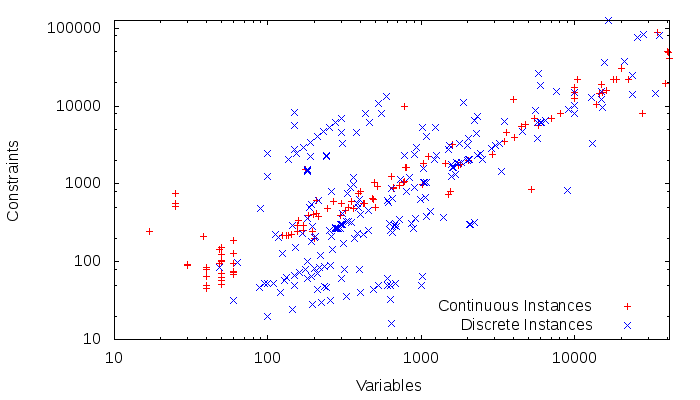
\includegraphics[width=0.85\textwidth]{pic_overview.png}
  \caption{...\label{fig:1}}
\end{figure}

%%%%%%%%%%%%%%%%%%%%%%%%%%%%%%%
\begin{figure}\centering
  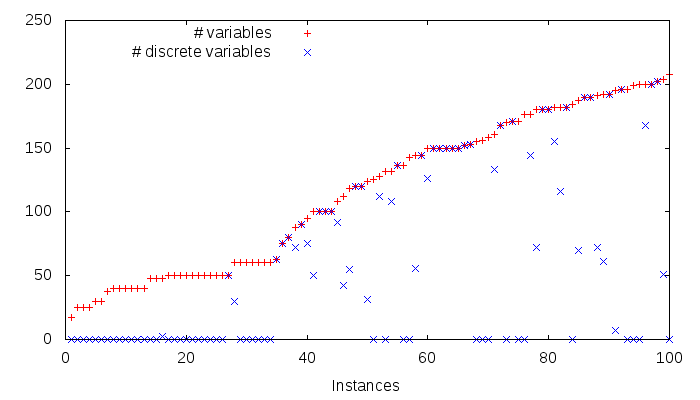
\includegraphics[width=0.85\textwidth]{pic_var_small.png}
  \caption{...\label{fig:4}}
\end{figure}

\begin{figure}\centering
  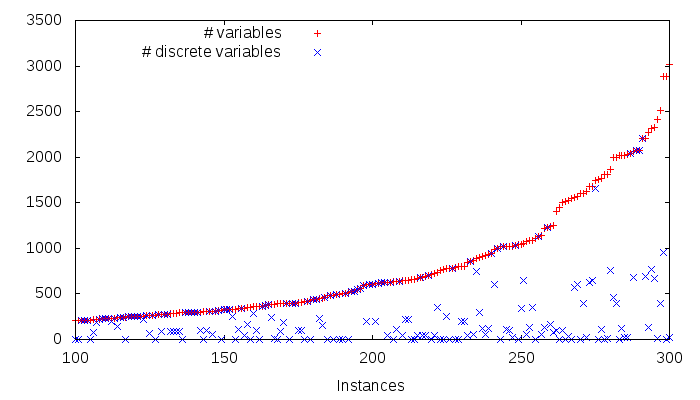
\includegraphics[width=0.85\textwidth]{pic_var_medium.png}
  \caption{...\label{fig:3}}
\end{figure}

\begin{figure}\centering
  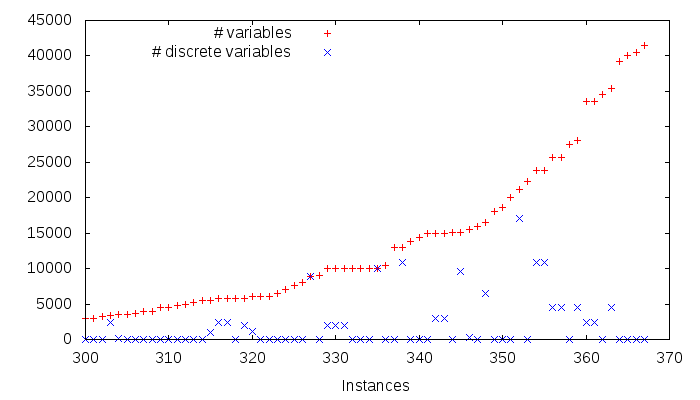
\includegraphics[width=0.85\textwidth]{pic_var_big.png}
  \caption{...\label{fig:2}}
\end{figure}

%%%%%%%%%%%%%%%%%%%%%%%%%%%%%%%%%%%%%%%
\begin{figure}\centering
  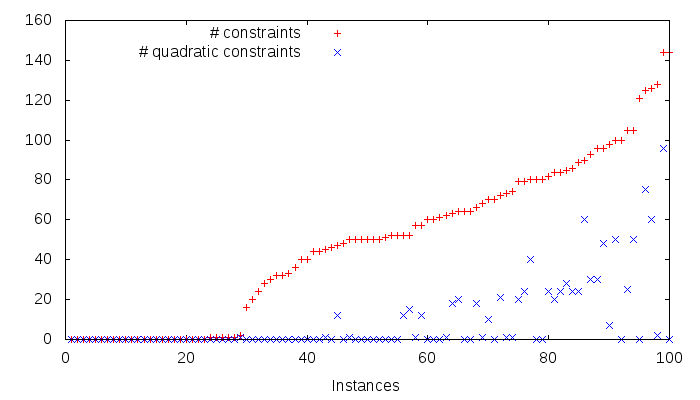
\includegraphics[width=0.85\textwidth]{pic_constr_small.png}
  \caption{...\label{fig:5}}
\end{figure}

\begin{figure}\centering
  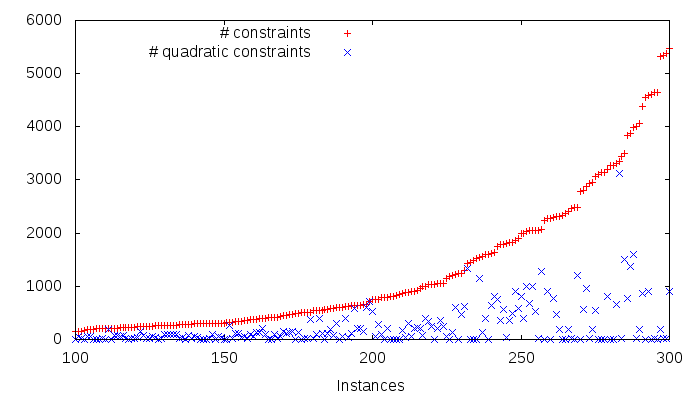
\includegraphics[width=0.85\textwidth]{pic_constr_medium.png}
  \caption{...\label{fig:6}}
\end{figure}

\begin{figure}\centering
  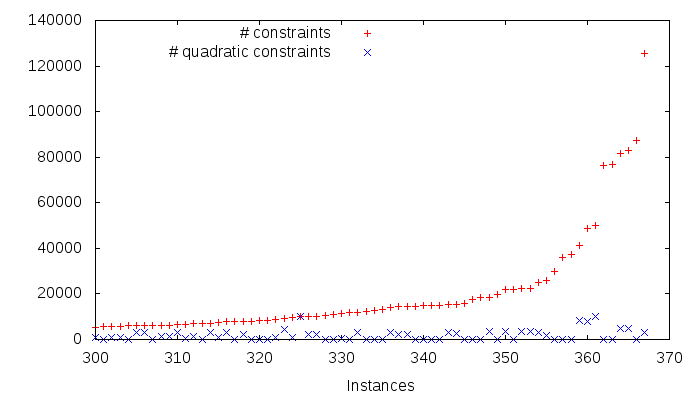
\includegraphics[width=0.85\textwidth]{pic_constr_big.png}
  \caption{...\label{fig:7}}
\end{figure}
%%%%%%%%%%%%%%%%%%%%%%%%%%%%%%%%%%%%%%%%%

\begin{figure}\centering
  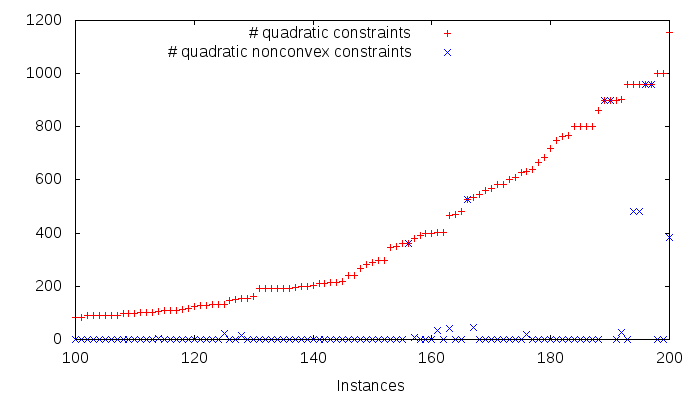
\includegraphics[width=0.85\textwidth]{pic_quad_vs_convex_constr.png}
  \caption{...\label{fig:8}}
\end{figure}
%%%%%%%%%%%%%%%%%%%%%%%%%%%%%%%%%%%%%%%%


\begin{figure}\centering
  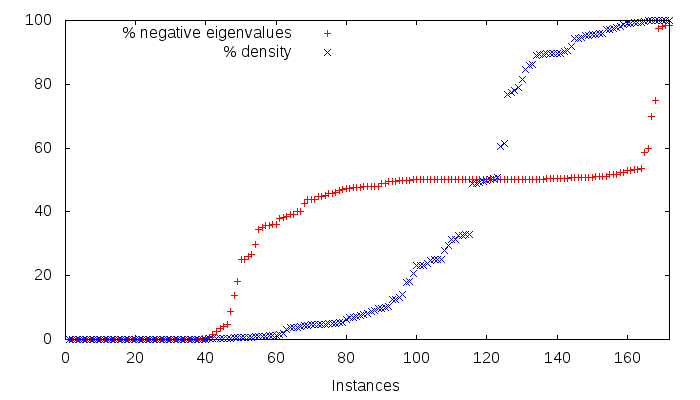
\includegraphics[width=0.85\textwidth]{pic_fuffa.png}
  \caption{...\label{fig:9}}
\end{figure}

\begin{figure}\centering
  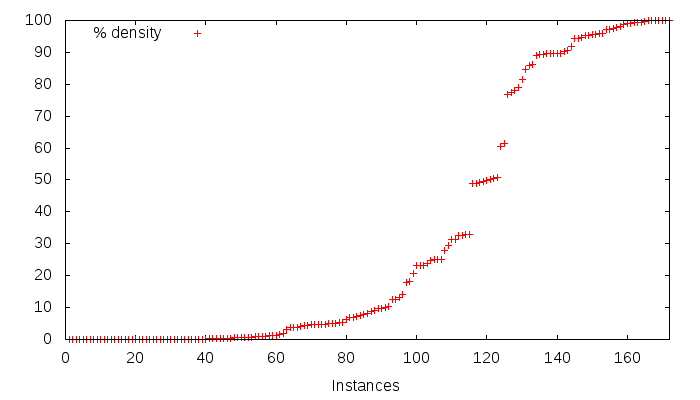
\includegraphics[width=0.85\textwidth]{pic_density.png}
  \caption{...\label{fig:10}}
\end{figure}

\begin{figure}\centering
  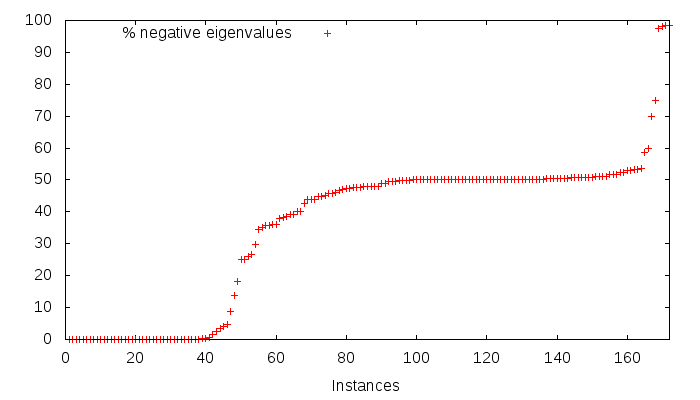
\includegraphics[width=0.85\textwidth]{pic_neg_eig.png}
  \caption{...\label{fig:10}}
\end{figure}









%- - - - - - - - - - - - - - - - - - - - - - - - - - - - - - - - - - - -
\subsection{Instance Selection}\label{subsec:selection}
\framebox{TASK X : write }










%- - - - - - - - - - - - - - - - - - - - - - - - - - - - - - - - - - - -
%- - - - - - - - - - - - - - - - - - - - - - - - - - - - - - - - - - - -
%  End QPLIB-3.tex
%- - - - - - - - - - - - - - - - - - - - - - - - - - - - - - - - - - - -
%- - - - - - - - - - - - - - - - - - - - - - - - - - - - - - - - - - - -
